\section{Demultipleksery}

\subsection{Symbol demultipleksera 4-bitowego}

\begin{figure}[h!]
    \centering
    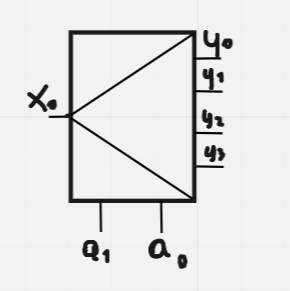
\includegraphics[width=0.4\textwidth]{images/dmux/dmux_s.png}
    \caption{Symbol demultipleksera}
    \label{fig:my_label}
\end{figure}

\subsection{Tabela prawdy}

\begin{figure}[h!]
    \centering
    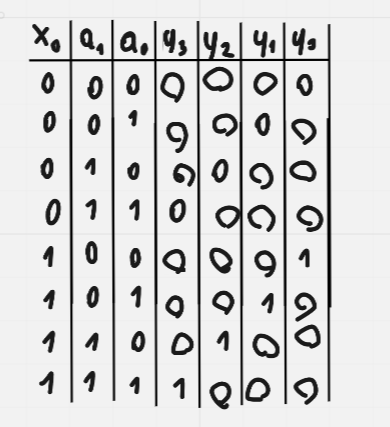
\includegraphics[width=0.45\textwidth]{images/dmux/dmux_t.png}
    \caption{tabela prawdy dla demultipleksera 4-bitowego}
    \label{fig:my_label}
\end{figure}

\newpage

\subsection{Siatka karnaugh dla demultipleksera 4-bitowego}

\begin{figure}[h!]
    \centering
    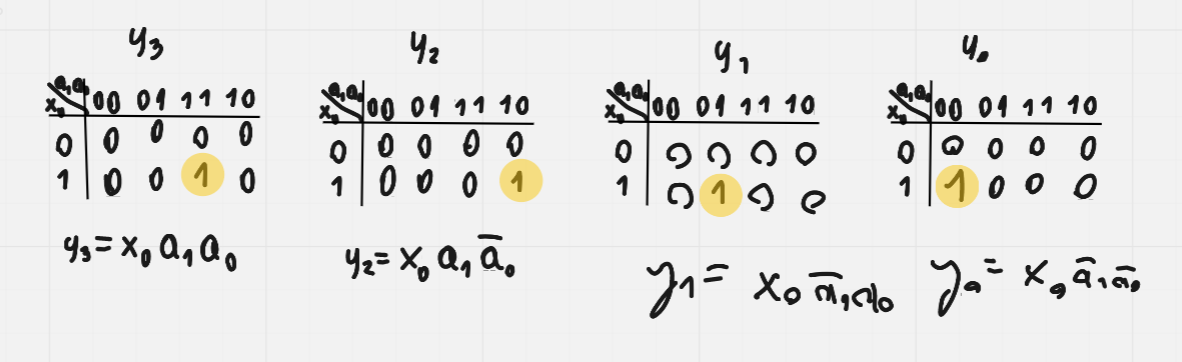
\includegraphics[width=0.8\textwidth]{images/dmux/dmux_k.png}
    \caption{siatka karnaugh}
    \label{fig:my_label}
\end{figure}

\subsection{Schemat układu}

\begin{figure}[h!]
    \centering
    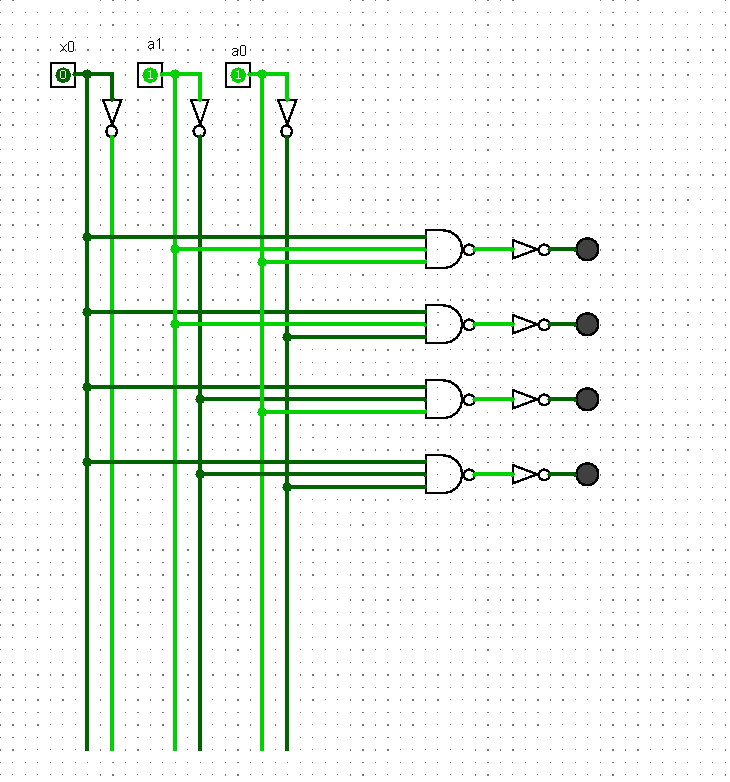
\includegraphics[width=0.7\textwidth]{images/dmux/dmux_l.png}
    \caption{schemat układu}
    \label{fig:my_label}
\end{figure}